\chapter{Einleitung}

In der modernen Arbeitswelt spielen flexible Arbeitszeitmodelle eine zunehmend wichtiger werdende Rolle, um den vielfältigen Anforderungen sowohl der Arbeitgeber als auch der Arbeitnehmer gerecht zu werden. 
Laut einer Studie der International Labour Organization wird Flexibilität in der Arbeitszeitgestaltung als entscheidender Faktor für die Vereinbarkeit von Beruf und Privatleben angesehen und kann die Zufriedenheit und Produktivität der Mitarbeiter signifikant erhöhen \cite[S.12 ff.]{ilo2018}. 
Ein zentrales Element dieser Flexibilität ist die Möglichkeit für Mitarbeiter, Schichten untereinander zu tauschen. 
Oft werden Schichttauschvereinbarungen privat organisiert, beispielsweise über Messenger-Dienste wie WhatsApp. 
%Problemstellung
In vielen Unternehmen organisieren Mitarbeiter ihre Schichtwechsel eigenständig und informell, oft über Messaging-Dienste wie WhatsApp. Dies gilt auch für die Mitarbeiter dieser Firma, die ihre Schichtwechsel in einer WhatsApp-Gruppe privat koordinieren. Ein typisches Beispiel einer solchen Liste für den Monat Januar sieht wie folgt aus:

\begin{figure}[h]
    \centering
    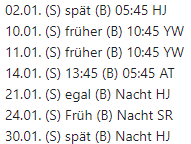
\includegraphics[clip,width=0.25\linewidth]{images/WhatsAppListe.png}
    \caption[Beispiel der Schichtwechsel-Liste aus WhatsApp für Januar]{Beispiel der Schichtwechsel-Liste aus WhatsApp für Januar}
    \label{WhatsAppListe}
\end{figure}

Hierbei steht (S) für „Suche“ und (B) für „Biete“, gefolgt von den jeweiligen Schichtzeiten und den Initialen der Personen.

Diese manuelle Methode bringt mehrere Herausforderungen und Ineffizienzen mit sich. Die fortlaufende Aktualisierung der Liste in WhatsApp führt oft zu einer unübersichtlichen Flut an Informationen, bei der Änderungen oder neue Einträge leicht übersehen werden können. 
Außerdem erfordert die aktuelle Methode von den Mitarbeitern, die gesamte Kommunikation und Liste in WhatsApp ständig zu überwachen, was zeitaufwendig und unpraktisch ist. Diese Herausforderungen beeinträchtigen die Effizienz der Schichtorganisation und führen zu mehr Unzufriedenheit bei den Mitarbeitern.

Das Ziel dieser wissenschaftlichen Arbeit ist es, ein benutzerfreundliches und effizientes UX Design Konzept zur Organisation von Schichtwechseln zu entwickeln. Dieses Konzept soll die aktuellen Probleme der ineffizienten WhatsApp-basierten Methode adressieren und eine strukturierte, leicht zugängliche und übersichtliche Alternative bieten.